\documentclass{config/apuntes}

\title{Minería de Textos}
\author{Sandra Mingo Ramírez}
\date{2025/26}
\acronym{MINTEX}

\usepackage[all]{nowidow}
\usepackage{listing}
\usepackage{color}
\usepackage{tabularx}
\usepackage{multirow}
\usepackage{makecell}
\usepackage{amsmath}
\usepackage{array}
\usepackage{soul}

\definecolor{dkgreen}{rgb}{0,0.6,0}
\definecolor{gray}{rgb}{0.5,0.5,0.5}
\definecolor{mauve}{rgb}{0.58,0,0.82}

\lstset{
  frame=tb,
  aboveskip=3mm,
  belowskip=3mm,
  showstringspaces=false,
  columns=flexible,
  basicstyle={\small\ttfamily},
  numbers=none,
  numberstyle=\tiny\color{gray},
  keywordstyle=\color{blue},
  commentstyle=\color{dkgreen},
  stringstyle=\color{mauve},
  breaklines=true,
  breakatwhitespace=true,
  tabsize=3
}

\usepackage{tocloft}

\advance\cftchapnumwidth 0.9em\relax
\advance\cftsecnumwidth 0.6em\relax
\advance\cftsubsecindent 0.5em\relax
\advance\cftsubsecnumwidth 0.5em\relax
\begin{document}

\begin{abstract}
La minería de textos, también conocida como minería de datos de texto, es el proceso de transformar texto no estructurado en un formato estructurado para identificar patrones significativos y nuevos conocimientos. Puede utilizar la minería de textos para analizar vastas colecciones de materiales textuales para capturar conceptos clave, tendencias y relaciones ocultas.
\end{abstract}

\pagestyle{plain}

\maketitle

\tableofcontents

%20/10 - Kostadin
\chapter{Introducción al lenguaje}
\section{Textos}

Los humanos nos comunicamos principalmente de forma oral, y el texto es la representación escrita de ese habla. Los animales también se comunican, usualmente sobre el estado actual o presente. El texto es una abreviación del habla, una forma de transcribirla con ciertas características:
\begin{itemize}
\item Es muy comprimido: el habla se produce mediante la acción de los músculos controlados por la corteza motora. Estamos limitados a emitir una cadena unidimensional de sonidos o fonemas.
\item Las categorías de sonido están acotadas y corresponden a los morfemas del lenguaje. Al escribir los morfemas, ya tenemos el texto.
\item El texto se transmite a través de letras, símbolos discretos.
\end{itemize}

El texto es una transcripción de una señal sonora que mantiene sus propiedades esenciales. Puede copiarse indefinidamente y es resistente al ruido.

El objetivo de la minería de textos es extraer información relevante de textos escritos. Algunos términos clave son:
\begin{itemize}
\item Información: Una letra es una unidad de información. Un dígito tiene menos opciones (0-9) comparado con las letras (a-z), por lo que posee menos información. Para codificar todo el abecedario se requieren al menos dos dígitos. La cantidad de información depende del número de posibles mensajes. Por ejemplo, con un dígito hay 10 posibilidades, con dos dígitos 100, y con tres dígitos 1000. En informática, se usan dos dígitos binarios (0 y 1). El logaritmo en base 2 mide la información en bits: 
$log_2(3) \approx 10$.
\item Relevancia: Algo es relevante si está relacionado con un problema específico. Por ejemplo, si buscamos una sustancia que cause diabetes en ratones, lo relevante es todo lo que se relacione con esa sustancia. La relevancia depende del problema concreto.
\item Fiabilidad: Debemos trabajar con información fiable, preferiblemente basada en la realidad y datos experimentales.
\item Texto humano: Tiene una estructura que viene de la secuencia continua de movimientos musculares al hablar. Además, existe una estructura jerárquica dada por la gramática y la sintaxis.
\end{itemize}

La redundancia garantiza robustez ante el ruido. El texto es redundante en varios niveles:
\begin{enumerate}
\item Fonemas: un fonema, como la vocal "a", tiene una duración corta (décimas de segundo). Si parte de la señal se pierde, otras repeticiones ayudan a comprenderlo.
\item Variaciones pequeñas en sonidos o escritura normalmente no afectan al significado. Por ejemplo, quitando las vocales, aún podemos entender un texto. Muchos lenguajes antiguos, como el árabe o los lenguajes semitas, no escriben vocales. Estas se introdujeron para facilitar la lectura sin conocer el contexto.
 \end{enumerate}

Ejercicio: estimar la velocidad de transmisión entre humanos de texto en dos contextos: uno escribe y el otro lo recibe; uno lee algo ya escrito como una novela. No se puede estimar la información, solo un límite superior a la información ("no más que x"). %Esto no hay quien lo entienda
\begin{itemize}
 \item Vídeo: 5 000 000 bits por segundo
 \item Teléfono: 3 000 bps
 \item Radio: 20 000 bps
 \item Leer (para uno mismo, en silencio): de media 200 palabras por minuto, unas 1000 letras por minuto. Siendo 6 bits la letra, 6000 bits por minuto o 100 bps.
 \item Escribir un texto: 60-90 palabras por minuto, con una media de 5 letras por palabra: 360-540 letras por minuto. Siendo 6 bits la letra, sale 40-60 bps
\end{itemize}

No toda comunicación es habla humana. Por ejemplo, si una persona describe algo para que otra lo dibuje, la información transmitida será muy diferente.
Tenemos diferentes tipos de señales: sonora o de letras. En términos de información, la función $f(x)$ tiene menos información que su argumento $x$, es decir, $f(x) < x$. 

\section{Artículos}
La mayoría de la información científica se encuentra en artículos. Un artículo es un texto publicado que puede incluir imágenes y fórmulas. Los artículos científicos y periodísticos se parecen: ambos tienen autores y reflejan la opinión de éstos. El artículo es una función de la información del evento, por lo que contiene menos información que el propio evento. Los autores están limitados por sus conocimientos y la fuente de información a la que acceden, como vídeos, relatos, testimonios, etc. El tiempo de escritura es también importante; el autor produce la mejor versión posible en ese momento, dentro de su contexto.

Un artículo de una página de periódico suele tener unas 300 palabras. Este valor puede obtenerse comprimiendo el contexto y el artículo.

En artículos científicos existe cierto grado de censura; no todo lo que sabe el autor se incluye. Cuanto más accesible es el artículo, mejor, por eso existen iniciativas OpenSource. Existen varios tipos de artículos científicos: investigación original, reviews (revisión de varios trabajos), propuestas metodológicas, estudios de caso (case studies, con potencia estadística limitada) y opiniones.

Un artículo cercano a la realidad contiene más información. Las fuentes más fieles incluyen historiales clínicos, diarios de laboratorio, datos estadísticos, comunicaciones entre personas sobre hechos, y datos del Internet of Things.

Actualmente, también están disponibles fuentes preprocesadas por inteligencia artificial (IA), que son modelos estadísticos del lenguaje. Reflejan la opinión prevalente, pero no su diversidad, tienen un horizonte temporal limitado, y un retraso por el tiempo de entrenamiento. Estas fuentes pueden reforzar opiniones dominantes debido a feedback positivo. Por ello, es recomendable complementar búsquedas IA con consultas directas a la web, aunque gran parte de la información en la web también ha pasado por IA.

\section{Minería de datos}
La minería de textos analiza uno o varios textos para responder preguntas como: ¿de qué trata? ¿Es fiable? ¿Tiene interés? ¿Qué información contiene y cómo describirla? ¿Cuál es la información nueva? ¿Cómo presentar la información de forma estructurada?
Los formatos estructurados incluyen bases de datos relacionales, no relacionales, grafos y programas.

Ejercicio: Food Insecurity Interventions to Improve Blood Pressure - JAMA Internal Medicine. 
El artículo tiene información no textual, está en los gráficos. Tiene 458 participantes, que está bien en cuanto a potencia estadística. 

Los \textbf{datos estructurados} tienen organización clara, fáciles de consultar, modificar y analizar, y suelen ser isomórficos con tablas relacionadas. Ejemplos: bases de datos, hojas Excel, gráficos conceptuales, datos de formularios.

Los \textbf{datos no estructurados} carecen de un modelo fijo, están en formatos naturales mezclando información útil con redundante, y no se pueden organizar trivialmente en tablas. Ejemplos: texto, vídeo, imagen.

El hipertexto es texto con relaciones internas o externas. Se estima que el 80\% de los datos son no estructurados.

\begin{figure}[h]
\centering
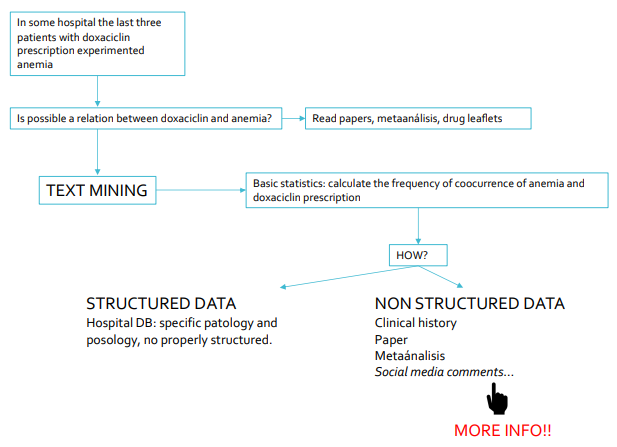
\includegraphics[width = \textwidth]{figs/ej-mineria.png}
\end{figure}

El trabajo fundamental en procesamiento de lenguaje natural es transformar datos no estructurados en estructurados. La idoneidad del método depende de la tarea real.
Dos grandes grupos de métodos:
\begin{itemize}
\item Métodos clásicos: dividir una tarea compleja en subtareas simples (p. ej. sistema de preguntas y respuestas basado en etiquetado POS, análisis sintáctico, reconocimiento de entidades nombradas) y combinarlas para generar la respuesta en lenguaje natural.
\item Métodos basados en aprendizaje profundo: un sistema único que procesa grandes cantidades de texto para crear una representación interna útil a la tarea.
\end{itemize}

\begin{figure}[h]
\centering
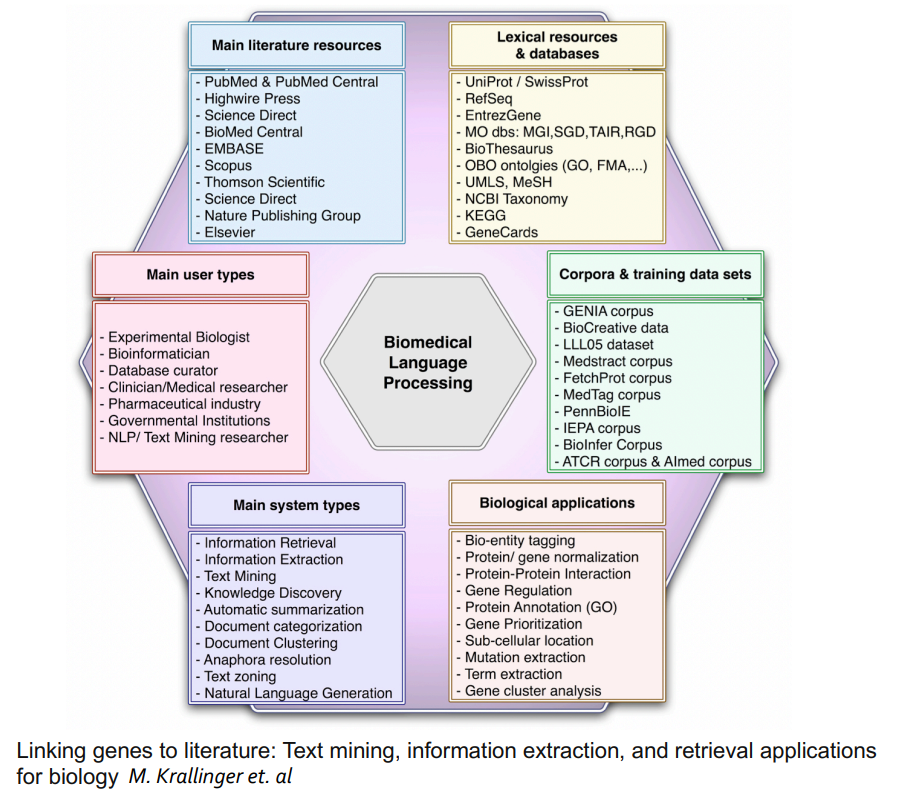
\includegraphics[width = 0.6\textwidth]{figs/blp.png}
\end{figure}

La pipeline del NLP funciona de la siguiente forma:
\begin{enumerate}
\item Extracción de datos de texto: Selección de las fuentes de datos de texto, aplicación de diferentes técnicas de consulta, API REST, extracción de datos web, consulta de bases de datos
\item Preprocesado: Formateo y estandarización de los datos de texto. Incluye tokenización, derivación, eliminación de palabras vacías y corrección gramatical.
\item Transformación de características: Transformación de los datos de texto en características procesables por ordenador.
Codificación N-gram, etiquetado POS, análisis sintáctico, agrupación Brown, vectores de palabras.
\item Generación del modelo
\item Análisis y tratado de resultados: estandarización, almacenamiento de los resultados
\end{enumerate}

\begin{figure}[h]
\centering
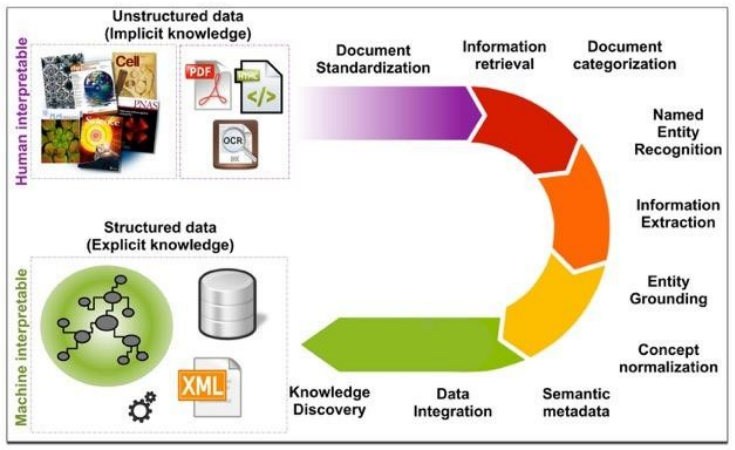
\includegraphics[width = 0.6\textwidth]{figs/biocuration.png}
\end{figure}

La biocuración es el proceso de recogida, verificación, organización y mantenimiento de datos biológicos para asegurar su calidad, coherencia y utilidad. En el contexto de la bioinformática, la biocuración implica seleccionar información relevante, estandarizarla y anotarla correctamente en bases de datos especializadas, facilitando así su análisis y reutilización en investigaciones científicas. El objetivo principal es transformar datos brutos en recursos confiables y estructurados que permitan realizar estudios precisos y reproducibles.

\begin{figure}[h]
\centering
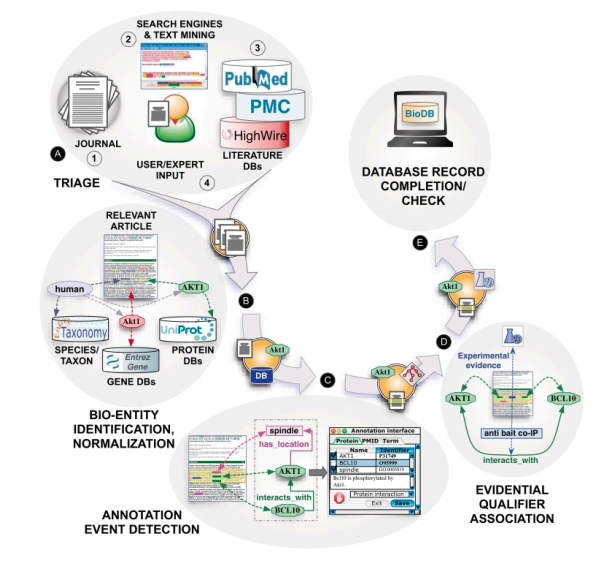
\includegraphics[width = 0.6\textwidth]{figs/biocuration2.png}
\end{figure}

Pese a la ayuda de la IA, la biocuración sigue siendo un proceso manual. Sus pasos son:
\begin{itemize}
\item Triaje: selección de artículos relevantes. El NLP clasifica el texto, detecta las entidades y tiene un aprendizaje no supervisado.
\item Normalización e identificación de bioentidades: hay varios nombres para una  misma patología, síntoma, causa, etc, por lo que se deben marcar como iguales. Por ejemplo: enfermedades vasculares hipertensivas, hipertensión e hipertensión arterial hacen alusión a lo mismo, pero con palabras distintas.
\item Anotación de eventos detectados: interacciones proteína-proteína, producción génica en cuanto a localización celular, etc, extracción de relaciones en general.
\item Asociación de calificadores probatorios
\item Comprobación y completar las entradas de la base de datos
\end{itemize}

Extraer relaciones entre entidades es una de las tareas más difíciles en
bioNLP. Es difícil porque, por un lado, es complicado extraer información significativa de la muestra para construir un modelo automático y, por otro lado, los modelos heurísticos no pueden abarcar todo el espectro de casos.

\subsection{Ontologías}
Más de 1500 bases de datos biológicas activas con datos y términos de diferentes campos y más de 200 vocabularios diferentes incluidos en recursos como UMLS: ontologías genéticas, secuencias genéticas, estructura proteica, terminología médica, taxonomías de especies, etc.

El UMLS (Unified Medical Language System) integra y distribuye terminología clave, normas de clasificación y
codificación, y recursos asociados para promover la creación de sistemas y servicios de información biomédica más eficaces e interoperables, incluidos los registros médicos electrónicos.

Originalmente integró 2 millones de nombres para unos 900 000 conceptos de más de 60 familias de vocabularios biomédicos, así como 12 millones de relaciones entre estos conceptos.
\begin{itemize}
\item Vinculación de términos con diccionarios estándar.
\item Exploración de ontologías de términos.
\item Búsqueda de relaciones entre términos.
\item Correspondencia entre uno y muchos de diferentes fuentes de bases de datos.
\end{itemize}

Los Medical Subject Headings (MeSH) son un vocabulario controlado y organizado jerárquicamente elaborado por la Biblioteca Nacional de Medicina. Se utiliza para indexar, catalogar y buscar información biomédica y relacionada con la salud.


%Exercise (5 min): Look at the repository PMC. Perform a query about the subject of the Jama article. Describe the structure of the query (righthadside window). Poner también la ontología MeSH
%22/10 - Paco Jurado
\chapter{Procesamiento de lenguaje natural}
\section{Procesado de lenguaje natural}
\subsection{Definición de PLN}
El procesamiento del lenguaje natural (NLP por sus siglas en inglés) son un conjunto de métodos para hacer el lenguaje humano accesible a los ordenadores. Así, permite una comunicación "natural" entre humanos y máquinas y mejora la comunicación entre humanos (por ejemplo por traducción).

La ciencia ficción ya mostraba desde finales de los 70 máquinas que podían hablar. 

\subsection{Desafíos del NLP}
El test de Turing lo desarrolló Alan Turing en 1950 para comprobar la capacidad de una máquina a mantener una conversación como si fuera un humano. El test se basa en un humano que "chattea" y debe distinguir si está hablando con otro humano o con una máquina. Si no lo puede distinguir, se considera que la máquina ha pasado el test de Turing. 

NLP es difícil porque los lenguajes humanos son ambiguos, ilimitados, diversos, difusos, más y menos articulados. Hay palabras polisémicas, el orden de las palabras afecta a su significado, expresiones hechas ("dame tu teléfono" no se refiere al dispositivo, si no al número). La ambigüedad sintáctica se puede dar por la sintaxis, referencias a pronombres, y aunque para los humanos sea fácil de detectar y forme la base de muchos chistes, a la hora de pasarlo a la máquina se convierte en un problema. 

A la hora de hacer las traducciones, depende la composición de palabras. Dos palabras que por separado tienen un significado, cuando están juntas pueden tener otro. 

\subsection{Interdisciplinariedad del NLP}
El NLP se basa en muchas disciplinas muy diversas. Están los \textbf{lingüistas}, que buscan analizar cómo funciona el lenguaje, los ingenieros en \textbf{machine learning} e \textbf{inteligencia artificial} para poder automatizar las tareas y crear programas complejos. En general, toda la \textbf{informática} presenta la base de los algoritmos utilizados en NLP.

Estas áreas son las que diseñan los primeros algoritmos, pero con el tiempo salen cuestiones \textbf{sociales y éticas} por sesgos sociales, como pueden ser los géneros al traducir del inglés al español (nurse se traducía sólo como enfermera, no salía la alternativa de enfermero).

\section{Aplicaciones prácticas}
Entre las aplicaciones del NLP se encuentran:
\begin{itemize}
\item Traducción automática: traducción de un texto de un idioma a otro en su significado (no palabra por palabra).
\item Obtención de información: dada una consulta en nuestro idioma, identifica los documentos y páginas relevantes para esa búsqueda. 
\item Extracción de información: se tienen documentos de texto que no están estructurados (en cuanto a información, no del texto) de los cuales se intenta extraer la información estructurada para una base de datos.
\item Respuesta a preguntas: responder automáticamente preguntas propuestas por humanos en base a la información ya almacenada.
\item Clasificación de texto: asigna categorías o tags a textos en base a su contenido.
\item Minería de opiniones y análisis de sentimientos: identificar, extraer, cuantificar y estudiar de forma sistemática los estados afectivos y la información subjetiva (a partir del contenido textual generado por los usuarios).
\item Sistema de diálogo: Un agente conversacional o chatbot es un sistema informático diseñado para conversar con un ser humano (a través de un canal de texto). Los asistentes virtuales/personales inteligentes pueden realizar tareas o prestar servicios a una persona basándose en órdenes o preguntas. Así se crearon los agentes de generación de lenguaje conversacionales como ChatGPT o Gemini. Estos algoritmos generan texto como lo haría un humano (o como se ha hecho previamente), y estos sí pasan el test de Turing.
\end{itemize}

\section{Niveles del análisis lingüístico y tareas NLP}
\subsection{El pipeline de NLP}
Para conocer un idioma, hay que manejar muchos niveles de análisis lingüístico: habla, fonética, ortografía, morfología, lexemas, sintaxis, semántica, pragmática, etc. 

\begin{figure}[h]
\centering
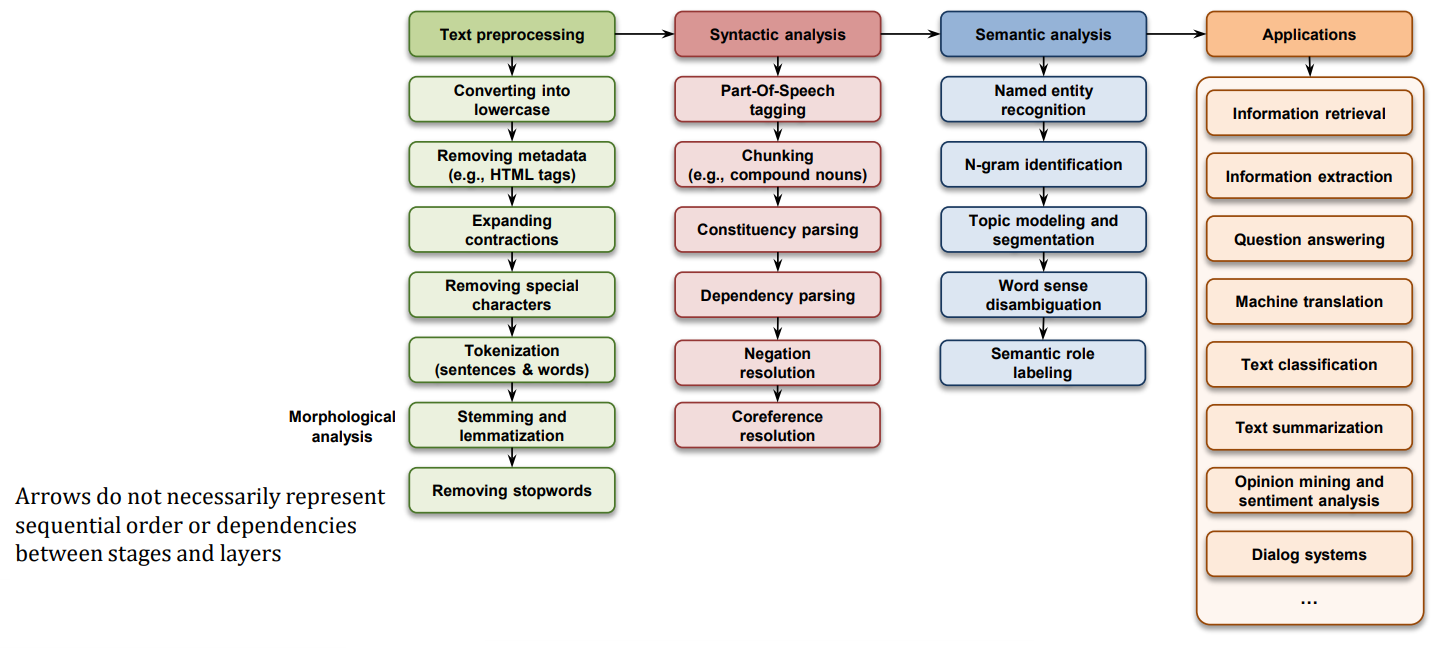
\includegraphics[width = \textwidth]{figs/nlp-pipeline.png}
\end{figure}

El primer paso es el \textbf{preprocesamiento} para normalizar todo (pasar a minúscula), quitar la metadata (tags, html), expandir las contracciones o los acrónimos, eliminar caracteres especiales, etc. También se eliminan las stopwords, que son palabras que no aportan nada de información, como los artículos o los verbos auxiliares. A continuación se stemiza y lematiza, es decir, se quitan las conjugaciones para obtener la raíz y obtener el lema (la palabra normalizada).

El siguiente paso es el \textbf{análisis sintáctico} donde se identifican las partes de la oración, se hace una composición de los grupos (nominales, preposicionales, etc) donde entra el análisis de constituyentes, resolución de dependencias y negaciones y se entra al \textbf{análisis semántico}. Con todo el procesamiento se pasan a las \textbf{aplicaciones}.

\subsection{Análisis sintáctico}
\paragraph{Part-Of-Speech (POS) tagging}
El POS tagging identifica para cada palabra o token si se trata de un nombre propio, verbo, determinante, etc. 

\paragraph{Parseo de constituyentes}
Las palabras tienen su POS tag y se van agrupando las estructuras sintácticas.

\paragraph{Parseo de dependencias}
Se extrae la estructura gramática de una oración, buscando la relación entre los constituyentes definidos previamente. 

\subsection{Análisis semántico}
\paragraph{Named Entity Recognition (NER)}
El reconocimiento de entidades se utiliza mucho en distintos contextos. Busca reconocer localizaciones, personas, lugares geopolíticos, números de teléfono, fechas, etc. Esto se puede utilizar posteriormente para la extracción de información. 

\paragraph{Resolución de co-referencias}
Se busca qué hace referencia a la misma entidad en un texto para reemplazarlo y que el procesamiento del texto sea igual. En ocasiones, es necesario completar la información (por ejemplo, una noticia de "el presidente ha dicho ...", si a la semana hay un cambio de gobierno).

\paragraph{Word Sense Disambiguation (WSD)}
En ocasiones, las palabras pueden hacer referencia a más de una cosa por ser polisémicas o tener otras ambigüedades, por lo que se deben desambigüar. Para ello se debe ver el contexto de la oración. Generalmente, se coge la palabra de la frase con menos alternativas de ambigüedades y a partir de ella se escogen las otras acepciones.

\paragraph{Etiquetado semántico}
Al hacer el etiquetado semántico, se le está poniendo cierta taxonomía para indicar las estructuras predicado-argumento como agente, predicado, tema y localización. Son representaciones abstractas de las funciones.

\section{Breve historia del NLP}
\subsection{NLP antes de la era Deep Learning}
Los inicios se deben a lingüistas y matemáticos. En los 1960s, se formalizan las teorías gramáticas. En los 90 se generan modelos estadísticos que permitieron identificar los stopwords en base a la frecuencia. Los modelos bayesianos funcionaban muy bien.

\subsection{NLP durante la era Deep Learning}
Los primeros modelos neuronales aplicados al lenguaje entraron en el 2003 y requerían una computación enorme. En los 2010 se crearon las GPU, por lo que el tratamiento matricial mejoró con creces. También entraron los word embedding, donde se obtenían representaciones vectoriales de los conceptos vinculados a las palabras con redes neuronales. Esto marcó un antes y un después. Se crearon distintas arquitecturas con los mecanismos de atención y transformer, y en 2020 los modelos grandes de lenguaje.

Muchos de los modelos creados antes de la era Deep Learning se siguen utilizando hoy día. Si por la tarea no se requiere una arquitectura deep, se pueden utilizar los modelos "clásicos". 
%22/10 - Paco Jurado
\chapter{El sentido de las palabras}
\section{Definiciones}
Hay palabras que tienen varios significados. Dado un lema o una palabra sin sus flexiones (en su forma más "normal") salen cada uno de las acepciones y significados. 

Un lema es una forma canónica de las palabras. Se coge la raíz y se añade lo pertinente para añadir el lema. Hay muchos algoritmos para obtenerlos, aunque son dependientes del idioma. Por ejemplo, en inglés se puede eliminar -ed o -ing para obtener el verbo sin conjugar. 

Las glosas son las definiciones. Esto no le sirve al ordenador, solo a nosotros al buscar un lema en el diccionario. 

Los homónimos son palabras que comparten una forma, pero tienen significados distintos. Banco puede ser la institución financiera o el asiento del parque, bat puede ser murciélago o bate. La homonimia se identifica en la extracción de información o question-answering, y viene en función del contexto. 

La polisemia es que una palabra pueda significar varias cosas relacionadas. La metonimia es la polisemia de forma sistemática. Por ejemplo, universidad puede ser el edificio o la institución. 

\section{Relaciones entre acepciones de palabras}
\subsection{Sinonimia y antonimia}
El sinónimo perfecto no existe, suele haber un matiz que los diferencie, ya que si no se hubiese abandonado una de las palabras. Hay veces que el contexto no permite intercambiar dos palabras. Por ejemplo, big y large, pese a ser sinónimos, sólo es correcto big en caso de "big sister". 

Los antónimos tienen significados típicamente opuestos. Ocurre similar que con los sinónimos, habiendo matices que hace que no sean antónimos perfectos. 

\subsection{Hipónimos e hiperónimos}
Los hipónimos son palabras que son más específicas que otras. Por ejemplo, coche es un hipónimo de vehículo, ya que es más específico. Hiperónimo es todo lo contrario, siendo una superclase más genérica. 

\subsection{Meronimia y holonimia}
La meronimia denota una parte de algo, y holonimia lo contrario. Por ejemplo, rueda y coche, u oveja y rebaño.

\section{WordNet}

WordNet es un tesauro o diccionario, una base de datos que representa las acepciones de palabras con versiones en distintos idiomas. Representa la relación entre los significados. 

Los sinsets (sets de sinónimos) son conjuntos de lemas que tienen la misma acepción y el mismo significado. Así, son equivalentes. Para una palabra polisémica se encontrará más de un sinset.

Las glosas son definiciones de texto humano que ayudan a entender el significado. Desde el punto de vista computacional interesa el sinset.

Los supersenses es una categoría de palabras  donde va indicando si algo es un acto, animal, artefacto, atributo, cuerpo, etc. Son unas superclases que pueden venir bien para la desambigüación.

WordNet permite encadenar las relaciones entre palabras para crear cadenas y llegar a una clase o palabra raíz. También nos proporciona clases de tipo instancia, como suele ocurrir con las ciudades. Con esto se podría construir un grafo para extraer toda la información de un documento. 

%27/10 
\section{Desambigüación del sentido de las palabras}
La desambiguación del sentido de las palabras (WSD) es la tarea de determinar qué sentido de una palabra se está utilizando en un contexto concreto. Tiene una larga trayectoria en la lingüística computacional y muchas aplicaciones. Busca proporcionar respuesta a preguntas como: «bat care» (¿El usuario es un vampiro? ¿O solo quiere jugar al béisbol?) o en traducción automática: traducción de «bat» como «murciélago» (animal) o «bate» (bate de béisbol) en español. Se ha utilizado como herramienta para evaluar modelos lingüísticos.

Hay varias aproximaciones:
\begin{itemize}
\item Basadas en el léxico: la idea es desambigüar algunas palabras mediante aprendizaje automático por el contexto.
\item Basado en todo el texto: en un lexicón con las diferentes acepciones (como Wordnet) se toma todo el texto y se busca la concordancia global, no palabra por palabra. Mapea las palabras input a los sinsets de WordNet, empezando por aquellas palabras con un solo sinset.
\end{itemize}

Hay que buscar líneas base. Algunos algoritmos cogen el \textbf{sentido más frecuente} para una palabra, escogiendo la acepción más comúnmente utilizada para cada palabra. Para WordNet esto se corresponde a la primera acepción, ya que está ordenado de mayor a menor frecuencia. Otra aproximación es un algoritmo con \textbf{un sentido por discurso}. Si todos los documentos o el discurso habla de animales, "bass" se vinculará al pez y no a la guitarra.

El \textbf{algoritmo de Lesk} se queda con la acepción en cuya glosas aparezcan palabras que también aparezcan en el texto que se quiera analizar. Esto se podría vincular también con las aproximaciones anteriores. Otros algoritmos utilizan embeddings, que son significados de palabras, y los muestra en un espacio n-dimensional. Así, se escogerá aquella acepción que se encuentre más cerca del vector de las demás palabras del texto. 

La Wikipedia es una fuente de información gigantesca. Saber si una palabra está vinculada con otra, se puede utilizar la glosa de la acepción, pero quizás es demasiado corta. Por ello, se puede ir a la Wikipedia y utilizar su contenido para desambigüar. 
%27/10 - Paco Jurado
\chapter{Part-of-Speech (PoS) Tagging}
\section{Parts of Speech (PoS)}
El PoS tagging identifica las propiedades gramaticales de una palabra: nombres, verbos, adjetivos, etc. La ventaja es que hay clases cerradas (determinantes, preposiciones, pronombres, etc) y estandarizadas, aunque también hay algunas clases abiertas como nombres, verbos, adjetivos y adverbios. 

Penn Treebank contiene el tagset para inglés de forma estandarizada. Tiene la nomenclatura ya establecida, asignando el tag DT a los determinantes, FW a las palabras extranjeras, IN a las preposiciones, etc. 

Alternativamente está el conjunto Universal Dependencies (UD) que tiene 17 PoS tags en lugar de los 45 de Penn Treebank. Estos tags se agrupan en tres clases (abierto, cerrado y otro). 

\section{El problema del PoS tagging}
El etiquetado del PoS consiste en asignando a cada palabra o token de un texto su función dentro de la oración. A partir de ahí se podría hacer el análisis sintáctico, semántico e incluso del discurso. 

Algunas de las aplicaciones son:
\begin{itemize}
\item Reconocimiento de entidades: nombres propios, lugar, organización, persona
\item Desambigüación de palabras: diferentes significados de palabras pueden tener distintas clases.
\item Traducción
\item Análisis de opinión
\item Preguntas a respuestas
\item Sistemas de diálogos
\end{itemize}

El PoS tagging no es trivial, ya que una palabra puede tener una etiqueta distinta en función de su contexto. Esto ocurre mucho en inglés donde se adjetivan los verbos con -ing, aunque también pueden ser gerundios. La mayoría de las palabras del vocabulario no es ambigüo y se sabe exactamente lo que significa, pero el 14-15\% restante proporciona la ambigüedad al texto. 

Se puede optar por un baseline y coger la más frecuente, y esto da una precisión alta, del 92\%. Otros algoritmos llegan hasta el 97\% cuando se trata del inglés con algoritmos como HMM o campos aleatorios condicionales. Entre las diferentes aproximaciones hay léxicas, basadas en reglas (si una palabra termina en -ed o -ing, puede ser un verbo), probabilísticas (HMM y CRF) y basadas en redes neuronales.

\section{PoS tagging probabilístico}
\subsection{Modelos ocultos de Markov (HMM)}
Las cadenas de Markov son modelos estocásticos que describen las probabildiades de secuencias de variables aleatorias (estados). La probabilidad de cada evento depende solo del estado que se ha dado en el evento anterior. La probabilidad de cada evento depende solo del estado en el que estamos y del evento. 

Las cadenas ocultas tienen una serie de estados que van a venir de situaciones observables (cada uno de los tokens o palabras) y hay unos estados ocultos que son la función de cada token dentro de la oración (la etiqueta). Así, están los estados o procesos no observados (ocultos) y los procesos observables (palabras del texto). Hay dos asunciones: (1) La probabilidad de un estado concreto depende únicamente del estado anterior. (2) La probabilidad de una observación de salida depende únicamente del estado que produjo la observación y no de ningún otro estado ni de ninguna otra observación

La matriz de transición de probabilidades representa la probabilidad de pasar de una etiqueta a otra. Si tenemos un verbo modal, lo más seguro es que a continuación venga el verbo principal, no un sustantivo. Luego se estima la maximum likelihood. 

La matriz de emisión de probabilidades representa las probabilidades asociadas a cada palabra dada la etiqueta. Multiplicando las dos matrices se puede calcular la probabilidad de la etiqueta de una palabra. 

Así, el proceso tiene dos etapas:
\begin{enumerate}
\item Decoding: dado un input de HMM como secuencia de observaciones, se encuentran los estados más probables de la secuencia. 
\item Codificación para PoS tagging: se elige la secuencia de etiquetas que van a estar vinculados a lo que se observa. Como se trata de un modelo generador, si la primera etiqueta es un nombre propio, generamos un nombre propio con cierta probabilidad. Esto no lo utilizamos nosotros, si no que aplicamos la regla de Bayes para usar las matrices de probabilidad de generación para identificar. 
\end{enumerate}

En definitiva, hay un texto de entrenamiento con las etiquetas ya asignadas previamente (corpus etiquetado) que se utiliza con las probabilidades para asignar las etiquetas a un texto nuevo. Así, la probabilidad de que aparezca una palabra depende únicamente de su propia etiqueta, y es independiente de las palabras y etiquetas vecinas, y la probabilidad de una etiqueta depende únicamente de la etiqueta anterior, en lugar de toda la secuencia de etiquetas (supuesto del bigrama).

Para encontrar la secuencia de etiquetas que maximiza la probabilidad de Bayes, se utiliza el \textbf{algoritmo de Viterbi}. Es un algoritmo de programación dinámica que va buscando la secuencia más probable dada una serie de palabras. Mira todos los recorridos y luego las palabras. Coge la primera palabra y asigna su etiqueta, y busca los posibles caminos a continuación. Ve la siguiente palabra y confirma el camino correcto de las posibilidades, y calcula las siguientes ramificaciones. 

\begin{figure}[h]
\centering
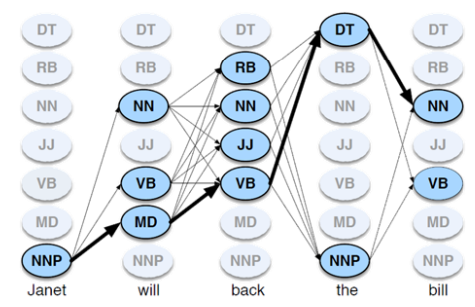
\includegraphics[width = 0.7\textwidth]{figs/viterbi.png}
\end{figure}

\subsection{Campos aleatorios condicionales (CRF)}
En los modelos ocultos de Markov, aprenden las etiquetas de un corpus para ahora generar etiquetas a un texto nuevo. Pero, ¿y si aparece una palabra que no estaba en el corpus? El algoritmo es fácil de implementar, pero es muy sensible cuando se altera el orden de las palabras y no haya aparecido al menos una vez en el corpus, ya que no se puede hacer la transición de los estados ocultos y no se va a reconocer como una secuencia válida. Aquí es donde entran los campos aleatorios condicionales.

Los campos aleatorios condicionales proporcionan resultados muy similares a las redes neuronales con menos maquinaria. No se utiliza un modelo generativo como en HMM, si no que se utiliza un modelo discriminativo. Se miran determinadas características de la palabra (por ejemplo, el lema y sufijos o prefijos, plurales, etc). Así, se buscan los atributos para cada palabra en una ventana de contexto específica (palabra + palabra anterior + palabra posterior, dos anteriores, dos posteriores, etc) y, en caso de que aparezca una palabra que no estaba en el corpus de entrenamiento, no pasa nada. Si acaba en -ed y tiene delante un nombre propio, con cierta probabilidad es un verbo porque se han visto patrones similares anteriormente, por lo que se etiqueta como tal. A través de las características se ve qué etiquetas no son y se discrimina así la etiqueta final. en HMM, se maximiza la probabilidad, y en CRF se discriminan todas las secuencias que maximizan la probabilidad.

Para cada palabra se define un modelo log-linear donde a cada uno de los atributos de la palabra se le asigna un peso. Aplicando unas fórmulas se llega a tener una probabilidad para la palabra. Se define una función que mapea las características de entrada a un determinado PoS tag. Se vuelve a aplicar el algoritmo de Viterbi, pero con las probabilidades calculadas a través de la CRF.

\section{PoS tagging basado en redes neuronales}
Los CRF siguen unas estructuras similares a perceptrones. Collins consiguió en 2012 una precisión del 97.1\% con Penn Tree utilizando un perceptron \footnote{Un perceptron es la red neuronal más simple. Recibe un input, realiza una transformación y saca un output. Si hay varias neuronas/perceptrones, se concatena.} estructurado y las características de current word, previous words, next words, previous tag y previous two tags, similar a las características empleadas en CRF.

\begin{figure}[h]
\centering
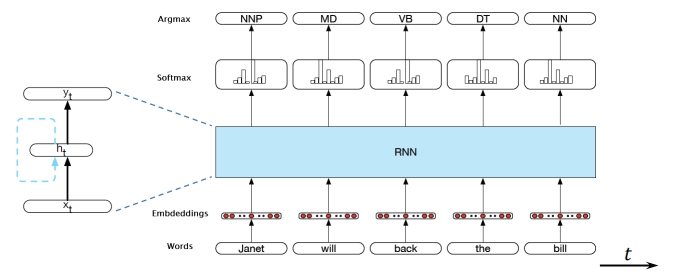
\includegraphics[width = 0.9\textwidth]{figs/rnn.png}
\caption{Red neuronal recurrente (RNN; recurrent neural network).}
\end{figure}

Entre una de las arquitecturas de las redes neuronales está la long short-term memory (LSTM). Es una red neuronal donde se van definiendo cómo están conectadas las neuronas y da un 95\% de precisión con CRF y 96.5\% con bi-LSTM (mira de izquierda a derecha y derecha a izquierda las palabras).
%27/10 - Paco Jurado
\chapter{Parseo de constituyentes}
\section{Lenguaje formal y constituyentes}
Hay dos formas de parseos: el parseo de constituyentes (forma de árbol) y análisis de dependencias (saltos a partir del verbo raíz para sacar las relaciones). 

\begin{figure}[h]
\centering
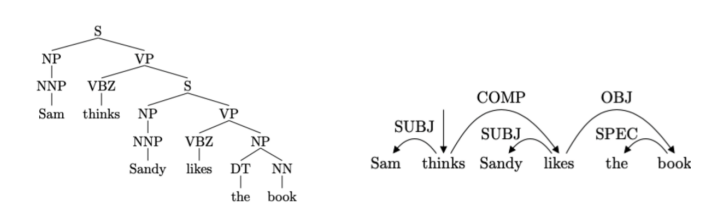
\includegraphics[width = \textwidth]{figs/parseo.png}
\end{figure}

La constitución sintáctica es la idea de que los grupos de palabras pueden comportarse como unidades únicas: constituyentes. Parte del desarrollo de una gramática implica crear un inventario de los constituyentes del idioma.

\section{Gramática libre de contexto}
La gramática libre de contexto o gramáticas de estructura sintáctica son el sistema formal más utilizado para modelar la estructura constituyente del inglés y otras lenguas naturales.

Un CFG consiste en un conjunto de reglas o producciones, cada una de las cuales expresa las formas en que los símbolos del lenguaje pueden agruparse y ordenarse, y un léxico de palabras y símbolos. 

El lenguaje formal definido por una CFG es el conjunto de cadenas que se pueden derivar del símbolo inicial designado. Cada gramática debe tener un símbolo inicial designado, que a menudo se denomina S. Dado que las gramáticas libres de contexto se utilizan a menudo para definir oraciones, S se interpreta normalmente como el nodo «oración», y el conjunto de cadenas que se pueden derivar de S es el conjunto de oraciones en una versión simplificada del inglés. 

Tenemos el lexicón con opciones de nombres, verbos, adjetivos, etc. Esos son los símbolos terminales. También hay reglas de producción: la frase está compuesta por nombre y predicado. El nombre puede ser un pronombre, nombre propio o determinante nominal. El predicado verbal puede ser verbo, verbo con nombre, verbo con nombre con preprosición, etc. Dado así un árbol construido con el análisis, se busca identificar si se ha podido generar con la gramática y los símbolos terminales. En esto consiste el análisis de la estructura de la oración. 

Las gramáticas libres de contexto vienen definidos por los signos no terminales.

\begin{figure}[h]
\centering
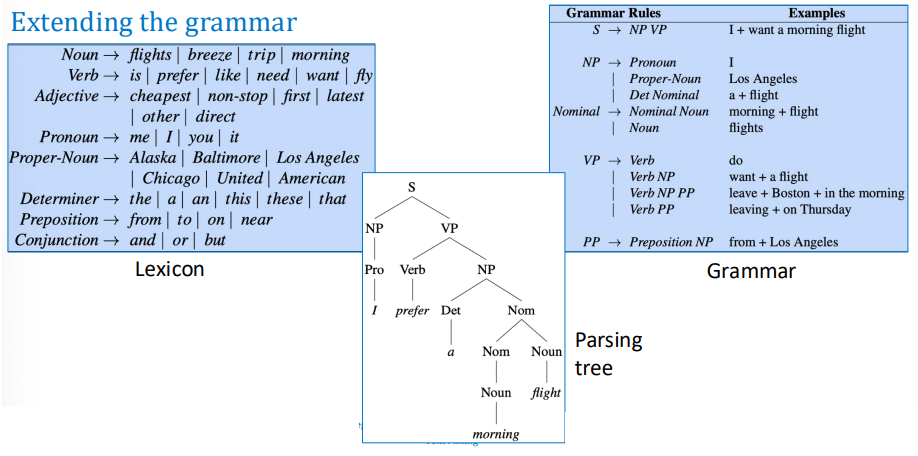
\includegraphics[width = 0.8\textwidth]{figs/grammar.png}
\end{figure}

\section{Parseo libre de contexto}
El parseo es la tarea de determinar si una cadena puede derivarse de una gramática libre de contexto dada y, en caso afirmativo, cómo. La estructura del análisis sintáctico puede responder a preguntas básicas del tipo «quién hizo qué a quién». Es útil para diversas tareas posteriores, como el análisis semántico, la traducción automática y la extracción de información.

Solo es posible realizar una búsqueda exhaustiva del espacio de análisis sintácticos recurriendo a supuestos de localidad. Estos permiten realizar búsquedas eficientes reutilizando subestructuras compartidas con programación dinámica.

El \textbf{algoritmo CKY} tiene un enfoque ascendente para el análisis sintáctico en una gramática libre de contexto. Comprueba de forma eficiente si una cadena pertenece a un lenguaje, sin enumerar todos los análisis sintácticos posibles. El algoritmo primero forma pequeños constituyentes y, a continuación, intenta fusionarlos en constituyentes más grandes.

El algoritmo va realizando las agrupaciones partiendo de los símbolos terminales de la oración (lo que estamos leyendo y recibiendo) y agrupa para ir creando los constituyentes. Para que funcione bien, las gramáticas no pueden estar escritas de cualquier modo; tienen que estar escritas en CNF, un símbolo no terminal que lleva a dos símbolos no terminales o a un símbolo terminal. Esto permite así agrupar de dos en dos.

\begin{figure}[h]
\centering
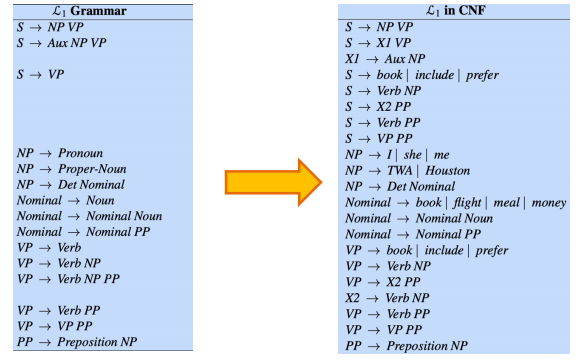
\includegraphics[width = 0.8\textwidth]{figs/cnf.png}
\end{figure}

\section{Gramáticas libres de contexto probabilísticas}
Se aplica la estadísitca para anotar las oraciones con treebanks y aprender modelos probabilísticos que infieran las reglas de producción. 

Se pueden utilizar gramáticas suficientemente robustas, compuestas por reglas gramaticales libres de contexto, para asignar un árbol sintáctico a cualquier oración. Esto significa que es posible construir un corpus en el que cada oración de la colección se empareje con un árbol sintáctico correspondiente. Este tipo de corpus con anotaciones sintácticas se denomina banco de árboles. Los bancos de árboles desempeñan un papel importante en el análisis sintáctico, así como en las investigaciones lingüísticas de los fenómenos sintácticos.

\begin{figure}[h]
\centering
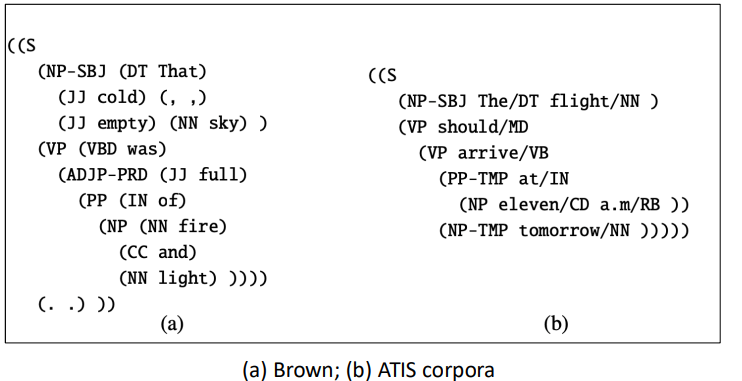
\includegraphics[width = 0.6\textwidth]{figs/treebank.png}
\end{figure}

Tenemos símbolos terminales (palabras), no terminales (constituyentes, PoS tag), reglas de producción, símbolo inicial y reglas de probabilidad. 

En las gramáticas libres de contexto, se agrupan dos a dos las reglas estrictas. Ahora, se hace lo mismo teniendo en cuenta la probabilidad de las reglas de producción. En otras palabras, se añade probabilidad al algoritmo CKY con argmax. 

\section{Evaluar parsers}
Para comparar los distintos enfoques de análisis sintáctico, necesitamos medir su rendimiento. Supongamos que tenemos un conjunto de análisis sintácticos de referencia (ground truth) etiquetados manualmente; por lo general, estos análisis sintácticos de referencia se extraen de un banco de árboles sintácticos como el Penn Treebank. Una solución sencilla sería la precisión por frase: el analizador se puntúa según la proporción de frases en las que el sistema y los análisis de referencia coinciden exactamente. La \textbf{métrica PARSEVAL} mide en qué medida los constituyentes del árbol de análisis hipotético se parecen a los constituyentes del análisis de referencia.

También se pueden utilizar recall y precisión. Un constituyente en un análisis hipotético Ch de una oración s se etiqueta como correcto si hay un constituyente en el análisis de referencia Cr con el mismo punto de inicio, punto final y símbolo no terminal. 

$$\text{labeled recall} = \frac{\text{\# of correct constituents in hypothesis parse of s}}{\text{\# of correct constituents in reference parse of s}}$$

$$\text{labeled precision} = \frac{\text{\# of correct constituents in hypothesis parse of s}}{\text{\# of total constituents in reference parse of s}}$$

La alternativa son las agrupaciones: El número de constituyentes para los que el análisis de referencia tiene un corchete como ((A B) C), pero el análisis hipotético tiene un corchete como (A (B C)).
%27/10 - Paco Jurado
\chapter{Parseo de dependencias}
\section{Problema del parseo de dependencias}
Una dependencia es una relación asimétrica sintáctica o semántica entre dos tokens léxicos. Un análisis de dependencias es el análisis de las relaciones entre las palabras del texto. Para ello, hay que tener un corpus etiquetado que diga que una palabra está relacionada con otra de una manera, etc. 

La idea es tener la relación sintáctica o semántica entre dos tokens. Siempre habrá relaciones de la cabeza a aquello que sea dependiente y el tipo de dependencia. Las dependencias están establecidas en Universal Dependency. Así, se crea un grafo en forma de árbol que empieza en el verbo principal y añade nodos entre tokens. 

Para cada palabra de la oración se intenta construir un grafo con las palabras o tokens del corpus y las relaciones de dependencia entre las palabras. La idea es tener una única cabeza (flecha que entra) a excepción de la raíz. Además, es un grafo conexo y acíclico. 

El corpus que esté etiquetado tiene para cada una de las palabras la etiqueta correspondiente. Algunos idiomas tienen algunas estructuras donde se dan cruces en el grafo. Si se pueden evitar a la hora de procesar, mucho mejor. 

El parseo de dependencias es una de las tareas del procesamiento de lenguaje natural donde se identifican las relaciones entre la cabeza y la palabra dependiente. El parseo es útil para traducción, extracción de información, etc, y suelen ser algoritmos rápidos. 

La proyectividad es que cada nodo dependiente se proyecta con un único nodo de la cabeza sin tener los cruces. Un árbol de dependencia es proyectivo si todos los arcos son proyectivos, es decir, ninguno se cruza. Si el grafo es proyectivo, será más fácil de implementar.

Existen limitaciones computacionales en las familias de algoritmos de análisis sintáctico de dependencias más utilizadas. Los enfoques basados en transiciones tienden a producir árboles proyectivos, lo que provoca algunos errores en oraciones con estructuras no proyectivas. Los enfoques de análisis sintáctico basados en grafos son más flexibles y capaces de abordar la limitación anterior.

\section{Algoritmos de parseo de dependencias}
\subsection{Parseo basado en transiciones}
En el \textbf{parseo basado en transiciones}, hay operaciones como desplazar y reducir que buscan relaciones de dependencia entre cada pareja de palabras. Se trata de una búsqueda codiciosa que encuentra óptimos locales, siendo así mejor para dependencias locales. Si el grafo es proyectivo, tiene $O(n)$, mientras que para los no proyectivos $O(n^2)$.

\begin{figure}[h]
\centering
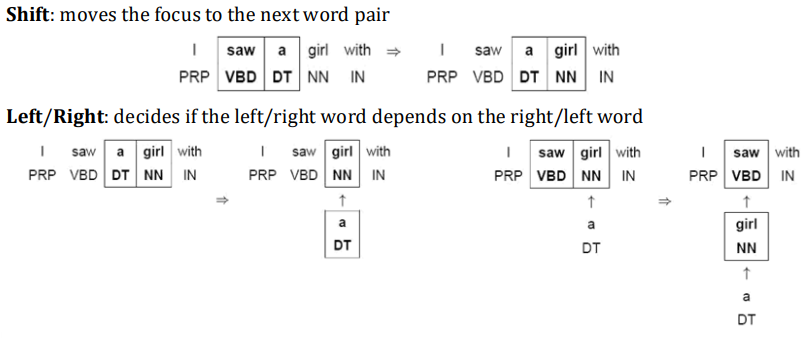
\includegraphics[width = 0.8\textwidth]{figs/transition.png}
\end{figure}

Se basa en un enfoque basado en pilas denominado «análisis sintáctico shift-reduce», desarrollado originalmente para analizar lenguajes de programación. Lo complicado del parseo no es construir la pila y el buffer, si no construir el oráculo o parser para que indique si dos palabras tienen dependencia para sacarlas de la pila y guardar la dependencia. 

\begin{figure}[h]
\centering
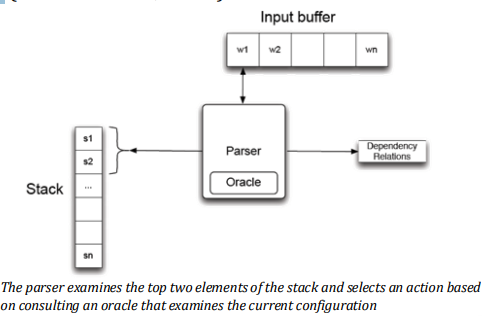
\includegraphics[width = 0.5\textwidth]{figs/transition-parser.png}
\end{figure}

El oráculo se crea con un algoritmo de aprendizaje automático o entrenando con un corpus. Así se van aplicando las relaciones encontradas.

\begin{figure}[h]
\centering
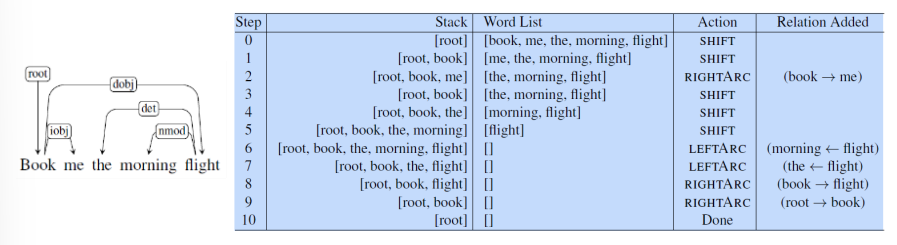
\includegraphics[width = \textwidth]{figs/transition-ej.png}
\end{figure}

\subsection{Parseo basado en grafos de dependencias}
Los \textbf{parseos basados en grafos} construyen un grafo completo con nodos dirigidos y con peso para encontrar el score más alta. Esta búsqueda es exhaustiva y encuentra el óptimo global. No importa si el grafo es proyectivo o no, pero el coste es de $O(n^3)$.

Se busca para maximizar las relaciones de dependencia con una métrica de score oportuna para la implementación. Entre las múltiples aproximaciones, está el \textbf{algoritmo de Chu-Liu-Edmond} que parte de una serie de premisas como grafo conexo, con peso y dirigido. Se pueden crear grafos más complejos con muchas relaciones de las que hay que decidir con cuál quedarnos.

\section{Evaluación de parsers}
Hay métricas a nivel de corpus y a nivel de oración. Hay métricas que ayudan a evaluar cuán bien funciona el parser, pero tampoco vamos a entrar en más detalle.

En resumen: tenemos el PoS tagging donde etiquetamos, el análisis de constituyentes y análisis de dependencias. Para cada uno de ellos necesitamos un corpus para entrenar y poder hacer el análisis posterior. Para cada análisis hay métricas que permiten evaluar el funcionamiento. PoS tagging es la entrada a los otros dos análisis. 

\end{document}
